\documentclass[8pt,a4paper,ngerman]{scrartcl}
\usepackage[utf8]{inputenc}
\usepackage{hyperref}
\usepackage{geometry}
\usepackage{graphicx}
\geometry{a4paper, top=20mm, left=30mm, right=30mm, bottom=30mm, headsep=10mm, footskip=12mm}

\begin{document}

% Silly header.

\begin{center}
    \LARGE{\textbf{Exposé zur Bachelorabeit}}
\end{center}
\begin{center}
    \large{Christopher Pahl}
\end{center}
\begin{center}
    \small{\today}
\end{center}

\section{Motivation}
    Heutzutage gibt es viele Plattformen die dabei helfen wollen neue Musik zu
    entdecken. Eine dieser Plattformen ist \url{https://www.last.fm}. User bekommen dabei
    basierend auf ihren Hörverhalten Vorschläge was sie als nächstes anhören
    könnten. Leider ist die Software (zum größten Teil) nicht OpenSource und zudem
    abhängig von den zentralen Servern des Betreibers. Daher wäre ein freies
    clientseitiges System wünschenswert.
    \\
    \\
    Die Zielgruppe wären hierbei Entwickler von Musicplayern oder vergleichbarer
    Software. Auch ein \emph{Standalone-Tool} wäre denkbar das von normalen Usern
    genutzt werden kann.

\section{Themenstellung}
    Erstellen einer Softwarebibliothek zur automatisierten Empfehlung von Musik
    basierend auf der Musiksammlung eines Nutzers und dessen Hörgewohnheiten.
    \\
    \\
    Im speziellen soll das System dabei die Musikdatenbank des Nutzers importieren
    können und dessen Hörgewohnheiten beobachten können. Daraus sollen dann
    Empfehlungen (\textit{N} ähnliche Songs zu Stück \textit{X}) und Dynamische Playlisten 
    (Playlist die zu den zuletzte Gehörten passt) abgeleitet werden können.
    \\
    \\
    Beteiligte Diszplinen der Informatik:

    \begin{itemize}
        \item Graphentheorie (Aufbau/Wartung der internen Graphenstruktur)
        \item Datamining-Algorithmen (Ähnlichkeitsmaß, Machinenlernende Systeme)
        \item Maschinelles Lernen (Prüfen ob Empfehlungen angenommen wurden)
        \item Audioanalyse (Moodbar (siehe Literatur [\ref{label_moodbar})])
    \end{itemize}

    \subsection{Namensgebung:}

        Die Library soll \emph{libmunin} heißen, wie Odin's Rabe \emph{Munin}:

        \begin{quote}
            \textit{Munin gehört zum altnordischen Verb muna (denken an, sich erinnern), 
            der Name Munin bedeutet folglich ,,die Erinnerung''.}
        \end{quote}

        Siehe auch: \url{http://de.wikipedia.org/wiki/Hugin_und_Munin}

\section{Geplantes Vorgehen}
    Es soll eine Prototyp in \emph{Python} implementiert werden. Sollte noch
    ausreichend Zeit bleiben (unwahrscheinlich) soll dieser Prototyp in eine
    \emph{C-Bibliothek} umgesetzt werden. Zuerst soll die Grundfunktionalität der
    Bibliothek stehen, danach können dann \emph{spezielle Provider}, welche
    beispielsweise eine \emph{Moodbar-Anaylse} oder \emph{Liedtexte vergleichen}, implementiert
    werden. Sollte die Library rechtzeitig in einem annehmbaren Zustand sein so soll
    die Library in einem \emph{MPD-Client zum Einsatz} kommen. 
    \\
    \\
    Später soll dann die \emph{Theorie} mit zuhilfenahme von \emph{Visualierungen} detailliert in 
    der Bachelor-Arbeit beschrieben werden und, nach Möglichkeit, wird das System an 
    \emph{echten Menschen} und verschiedenen Musiksammlungen getestet um zu sehen ob das
    System auch praxistauglich ist.


\section{Aufteilung/Zeitplanung}
    \paragraph{Projektarbeit:}
        \begin{enumerate} 
            \item Implementierung von \emph{libmunin} (55\%)
            \item (Optional) Beispielanwendung in einem MPD-Client (vorraussichtlich
                ,,\emph{Moosecat}'') (15\%)
        \end{enumerate}

    \paragraph{Bachelorarbeit:}
        \begin{enumerate} 
            \item Beschreibung der Theorie/Algorithmik mit Visualisierungen. (25\%)
            \item (Optional) Test mit echten Nutzern und verschiedenen
                Musiksammlungen. (5\%)
        \end{enumerate}

\section{Literatur}
    \begin{enumerate}
        \item \textit{Moodbar} \url{http://cratoo.de/amarok/ismir-crc.pdf} \label{label_moodbar}
        \item \textit{A Mood Based Music Classification and Exploration System} (\url{http://www.google.de})
        \item \textit{Automatic Playlist Generation via Music Mood Analysis} (\url{http://www.google.de})
        \item \textit{Polysound} \url{http://grupoweb.upf.edu/~luca.chiarandini/personal/v0/index.html#projectsPolysound}
    \end{enumerate}

% End of normal Text.
% Image down there:

\newpage

\begin{figure}[p]
    \vspace*{-2.0cm}
    \makebox[\linewidth]{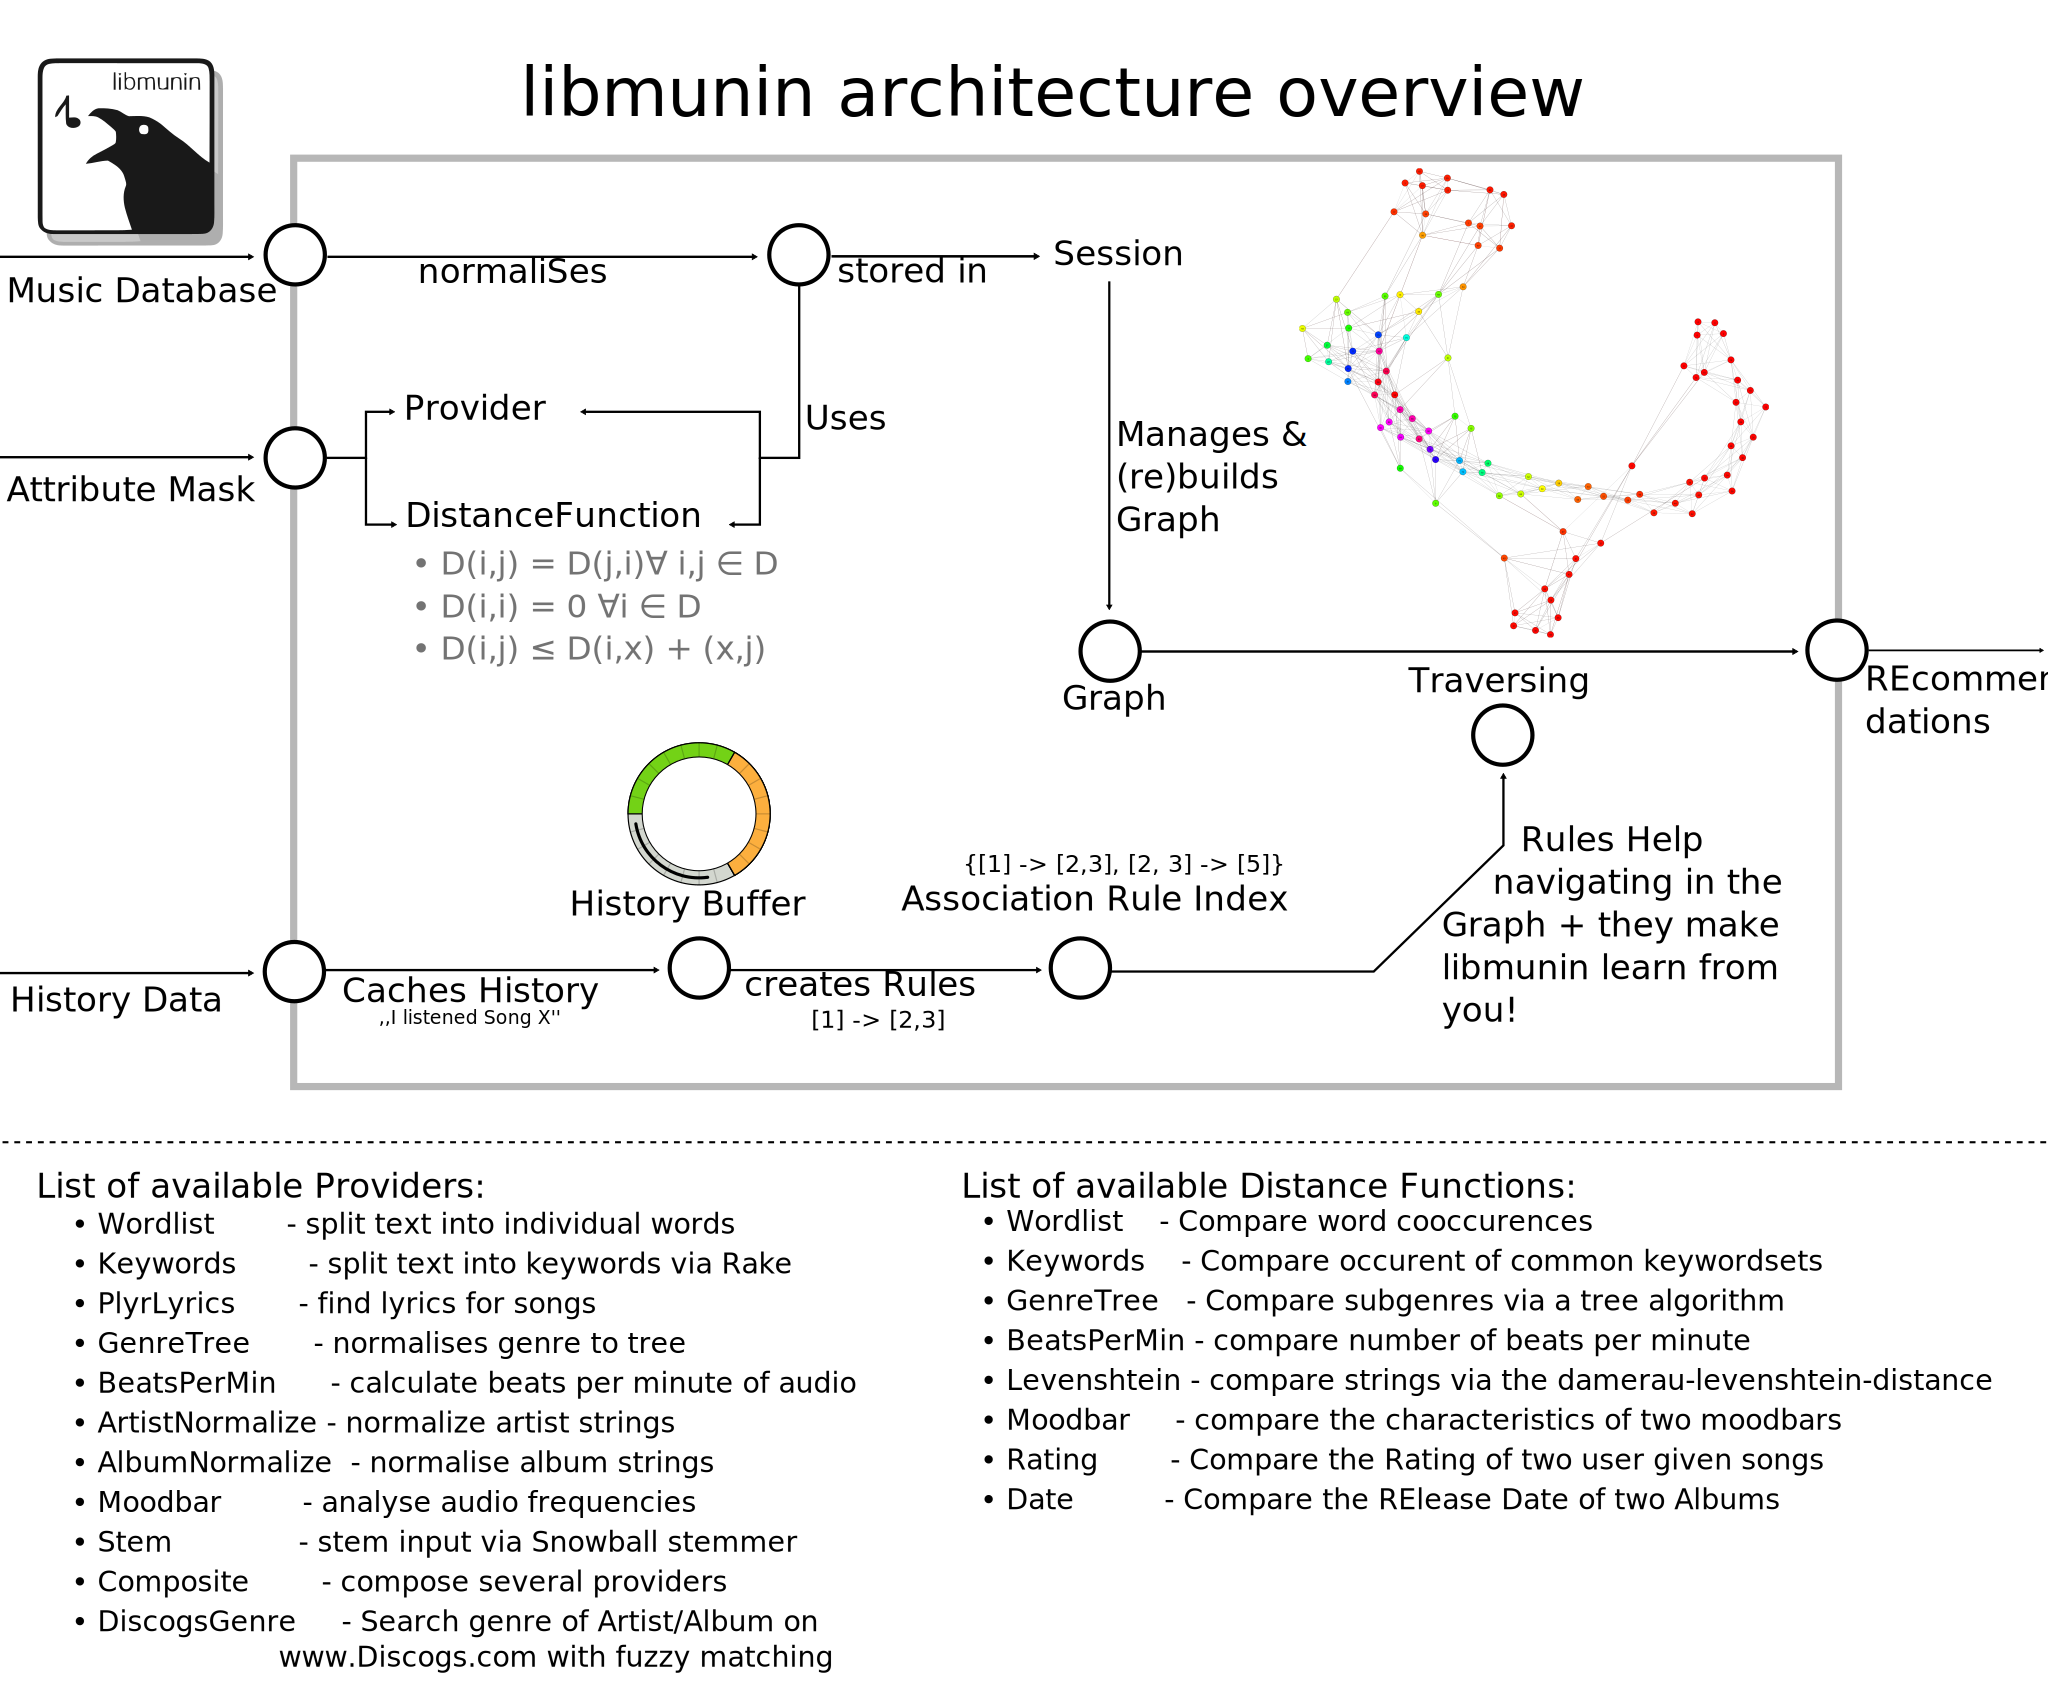
\includegraphics[width=1.41\linewidth]{arch.pdf}}
\end{figure}

\end{document}
